\section{The logistic equation of growth, saturation and diffusion}

\subsection{The logistic equation}

Growth and saturation in an environment with competition for limited resources.
The size of a population, with competition for limited resources, grows according to
a very specific process. It has an $S$-shape.

\subsubsection{Mathematical formulation}

Logistic differential equation:
\begin{align*}
    \frac{dP}{dt} = r P(t) \eckigeklammer{1 - \frac{P(t)}{K}}
\end{align*}
In the beginning ($P(t) << K$), for small $t$, we have exponential growth.
Later $P(t)$ plateaus and reaches the constant value of $K$.

\subsubsection{Mathematical solution}

With $P_0$ the initial population ($P(t=0)=P_0$). The solution, called
logistic function, is:
\begin{align*}
    P(t) = \frac{K P_0 e^{r t}}{K + P_0 (e^{r t} - 1)}
\end{align*}

\subsubsection{Different representations of logistic growth}

\begin{figure}[h]
    \centering
    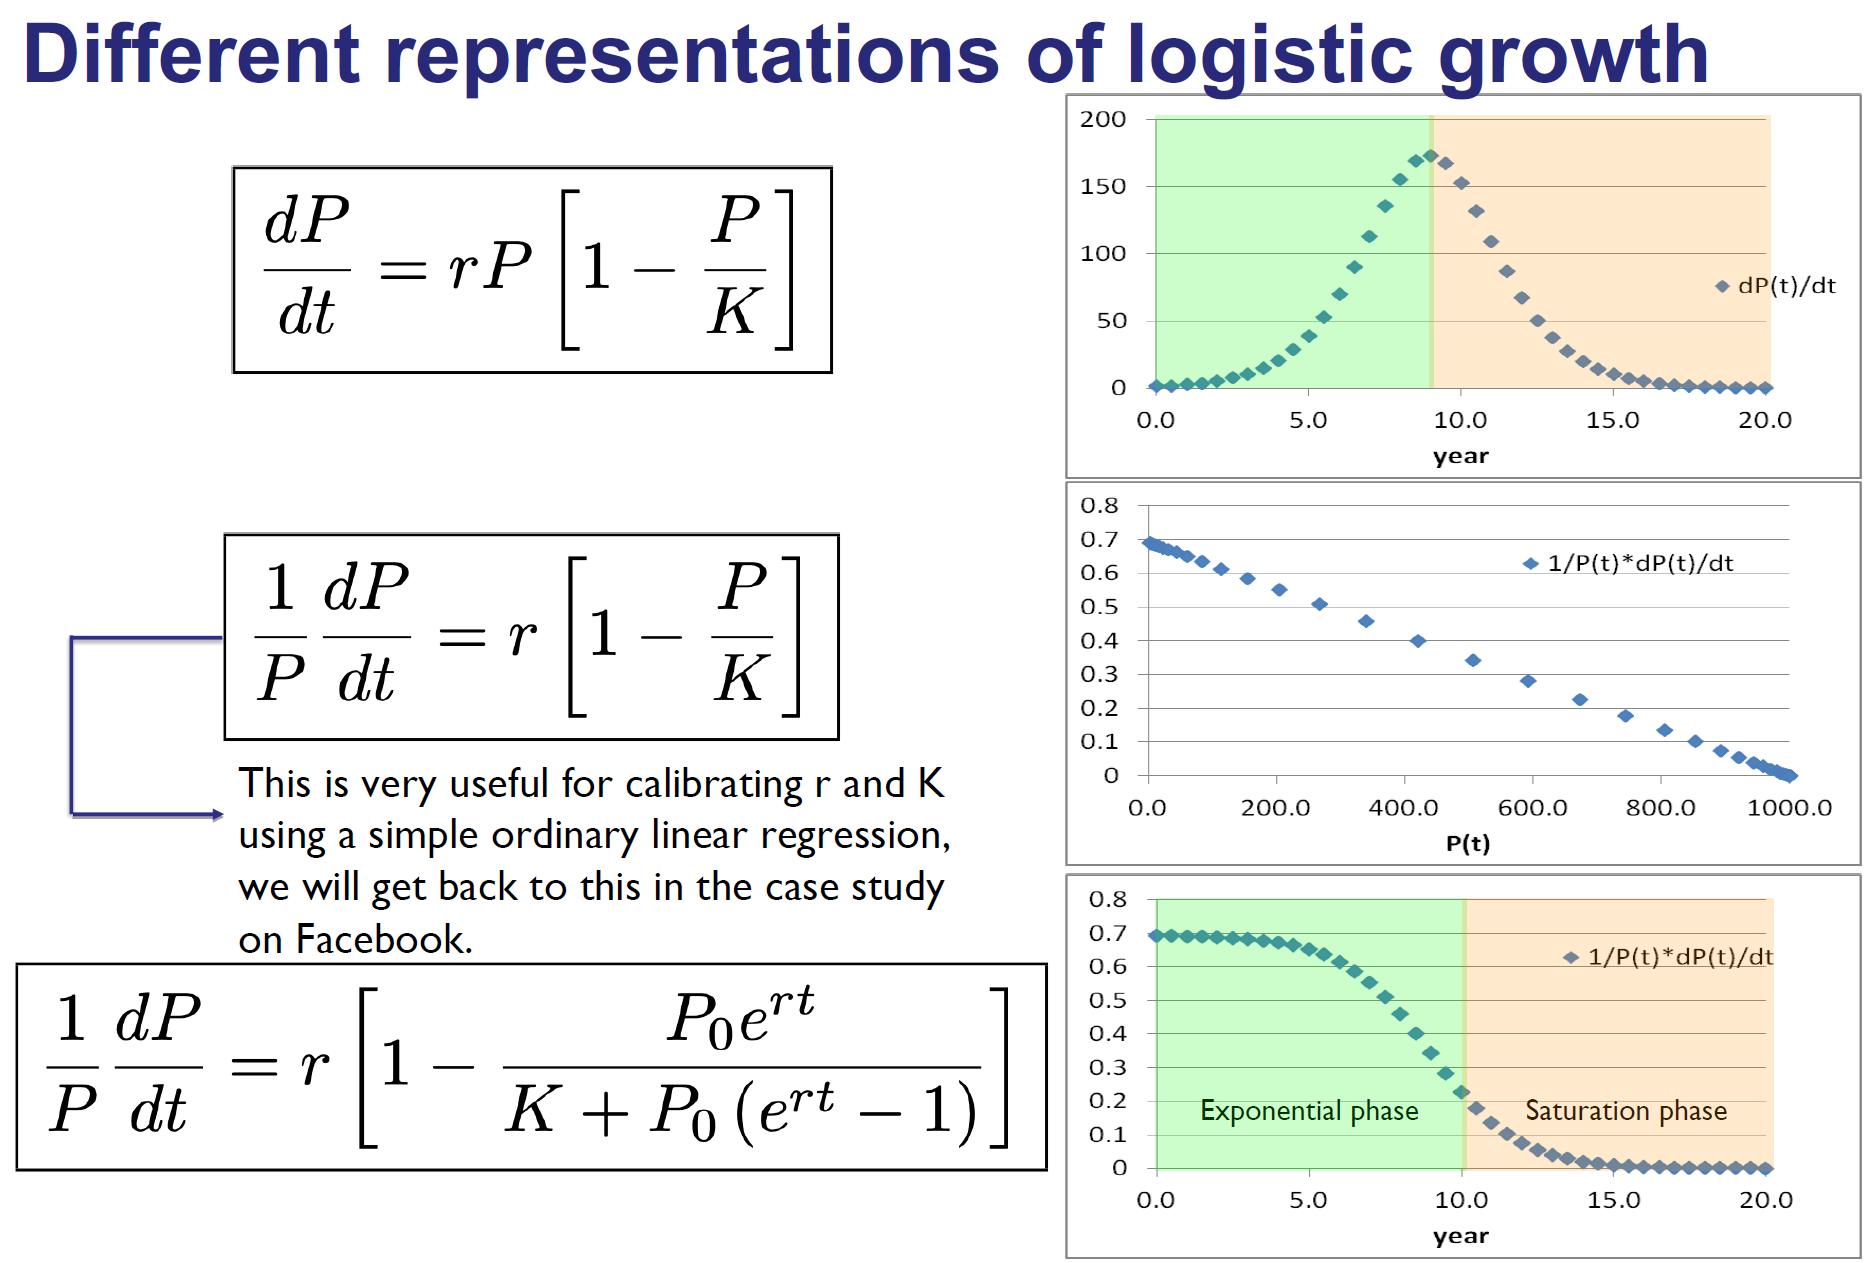
\includegraphics[width=0.6\textwidth]{Pictures/log_growth_diff_rep.png}
\end{figure}

\subsubsection{The Hubbert model and peak oil}

Oil production rates, in Gb/Year (billion barrels per year) were modelled using
the following equation:
\begin{align*}
    \frac{dP}{dt} = \frac{A}{1 + \cosh \eckigeklammer{-B (t-C)}}
    \hspace{10pt} \Rightarrow \hspace{10pt}
    P(t) = \frac{2 A}{B} \frac{1}{1+e^{-B(t-C)}}
\end{align*}
This is equivalent to the logistic equation, or that we referred to as the Varhulst
Growth Model, with
\begin{align*}
    K = \frac{2A}{B}
    \hspace{10pt} , \hspace{10pt}
    r = B
    \hspace{10pt} , \hspace{10pt}
    P_0 = \frac{K}{1 + e^{BC}}
\end{align*}

\subsubsection{Two types of models to describe epidemics}

\paragraph{Phenomenological models}

An empirical approach without a specific basis on the physical laws or mechanisms
that give rise to the observed patterns in the data. Emphasize the reproducibility
of empirical observations using simple models.

\paragraph{Mechanistic models}

Incorporate key physical laws or mechanisms involved in the dynamics of the
problem under study (e.g. population or transmission dynamics) in order
to explain patterns in the observed data. Often formulated in terms of a dynamical
system describing the spatial temporal evolution of a set of variables and are useful
to evaluate the emergent behaviour of the system across the relevant space of parameters.

\subsubsection{Population growth - Exponential}

\begin{itemize}
    \item Population increases in proportion to their size
    \item E.g. at a $10 \%$ annual rate if increase
        \begin{itemize}
            \item a population of 100 adds 10 individuals in one year
            \item a population of 1000 adds 100 individuals in one year
        \end{itemize}
    \item Allowed to grow unchecked, populations growing at a constant
        rate will rapidly approach infinity.
    \item This is known as exponential growth $C_t = C_0 e^{r t}$ where $C_t$
        is the population size, $r$ is the instantaneous (per capita) rate of
        increase and $t$ is time.
\end{itemize}

\subsubsection{Generalized growth model}

We can relax the assumption of exponential growth via "scaling of growth"
perameter $p$:
\begin{align*}
    \frac{dC}{dt} = r C^p (t)
\end{align*}
where $\frac{dC}{dt}$ describes the incidence growth phase over time $t$, the
solution $C(t)$ describes the cumulative number of cases at $t$.
\begin{itemize}
    \item $p=0$: this equation describes constant incidence over time and
        cumulative number of cases grows linearly.
    \item $p=1$: well-known exponential growth model.
    \item $0<p<1$: sub-exponential (e.g. polynomial) growth patterns.
    \item $1<p$: super exponential growth leading to finite-time singularity.
\end{itemize}

\subsubsection{Extension of Logistic type model}

\begin{itemize}
    \item Generalized-logistic growth model (GLM):
        \begin{align*}
            \frac{dC}{dt} = r C^p \klammer{1 - \frac{C}{K}}
        \end{align*}
    \item Richards model:
        \begin{align*}
            \frac{dC}{dt} = r C \klammer{1 - \klammer{\frac{C}{K}}^\alpha}
        \end{align*}
    \item Generalized Richards model (GRM):
        \begin{align*}
            \frac{dC}{dt} r C^p \klammer{1 - \klammer{\frac{C}{K}}^\alpha}
        \end{align*}
    \item The two additional parameters introduced:
        \begin{itemize}
            \item Parameter $p \in [0,1]$, describes the "scaling of growth"
                as in the generalized growth model and allows for sub-exponential
                growth during the early stage of the growth.
            \item Parameter $\alpha \geq 0$ measures the extent of deviation from the
                S-shaped dynamics of classical logistic growth model. Controls
                asymmetry.
        \end{itemize}
\end{itemize}

\pagebreak

\subsection{Generalized logistic growth modeling of the Covid-19 outbreak}

Plots can be seen in the Lecture slides of Lecture $5$.

\begin{figure}[h]
    \centering
    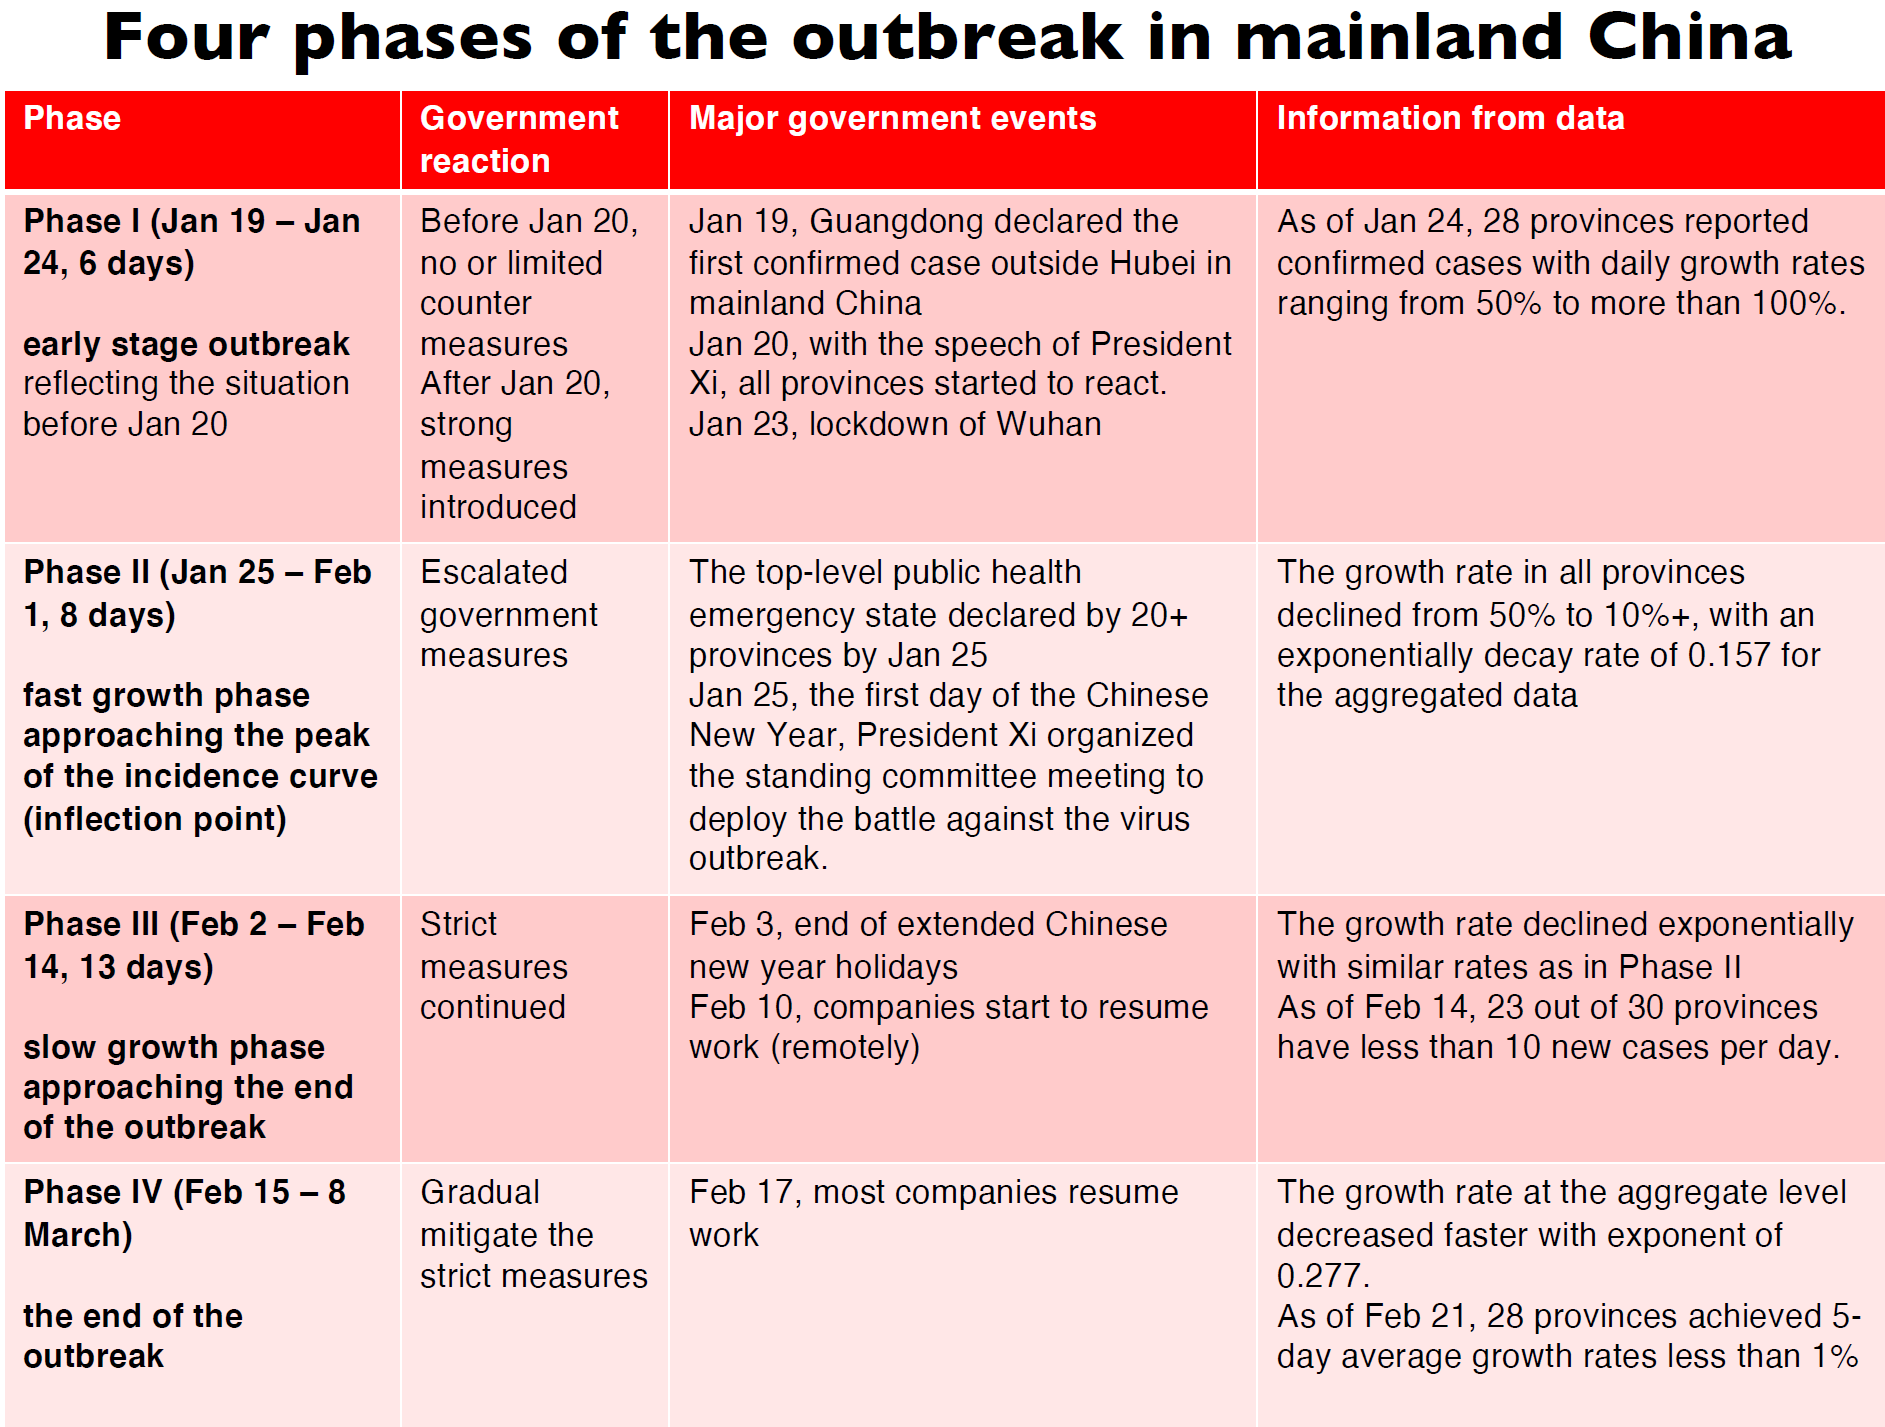
\includegraphics[width=0.9\textwidth]{Pictures/four_phases_of_the_outbreak_in_mainland_china.png}
\end{figure}

\begin{itemize}
    \item For countries in the early or middle stage of the outbreak, GRM is too
        flexible. Thus we consider the three simpler models with fewer parameters:
        the classical Logistic growing model, the Generalized-logistic growth model
        (GLM), and the generalized growth model.
    \item The classical Logistic growing model and Generalized-logistic growth
        model (GLM) tend to underestimate the number of infected cases, and the
        generalized growth model tend to overestimate the number of cases, which
        nicely serve as positive and negative scenarios for the future developments.
\end{itemize}

\paragraph{South Korea approach}

\begin{itemize}
    \item Korea doesn't have a tech solution, they have a solution that uses tech.
        It's different. When it comes to contact tracing, Korea didn't reinvent the
        wheel. They just used technology to dramatically speed it up. The Korean
        system allowed them to trace contacts in as little as $10$ minutes, which
        is unheard of. It's like everyone else is on bicycles and Korea has a bullet
        train.
    \item Everyone's talking about apps. Get everyone to install an app and, boom,
        contact tracing. That's not how it works. Korea did not rely on an app for
        contact tracing. Instead of an app, they used a wide constellation of data
        a board, redundant set of data combed over by trained people.
    \item One key insight is speed. All of their technology, all of their
        bureaucracy is just there to make their response as fast and agressive
        as possible. That's the only way to beat an exponential disease.
\end{itemize}


\paragraph{Summary}

\begin{itemize}
    \item Ultimately, the Covid-19 pandemic is a low-level stressor (anyone can
        imagine much worse stressors) BUT the consequences will be severe and
        disproportionate due to the mismanagement and unbalanced monodimensional
        responses.
    \item The guiding principle of our time: CYA (cover your ass) (active
        throughout time but now in "hyper-drive") Hyper-judicialization
        (appearing to save lives now is what counts)
    \item CYA explains the response of governments, Italy following China, and
        the rest of Europe (except Sweden) following Italy.
    \item In a society that aims at the mirage of "zero risk", lack of courage
        to follow a course of action and management based on scientific knowledge.
    \item Developing real-time research to inform decisions is like trying to
        develop GPS in the time of the sextant. Research takes time.
    \item $\Rightarrow$ considerable increase of uncertainties catalyzed by normal
        conflicts between scientists.
    \item This amounts to a devastating failure of leadership and courage.
\end{itemize}


\subsection{Generalization of logistic equations}

\begin{enumerate}[]
    \item \underline{Observation}: many systems exhibit succession of $S$-curves
        because advances in technology etc. increase the carrying capacity $K$.
    \item \underline{Idea}: include this into the logistic equation with a
        population dependent carrying capacity with delay time $\tau$.
        \begin{align*}
            \frac{d P}{d t} &= r P(t) \eckigeklammer{1 - \frac{P(t)}{K(t)}}
            \hspace{15pt} \text{with} \hspace{15pt}
            K(t) = A + B P(t - \tau)
            \\
            \Rightarrow
            \frac{d x}{d t} &= x(t) - \frac{x^2(t)}{a + b x(t - \tau)}
        \end{align*}
        with $x \sim P$ and parameters $a,b$ related to $r,A$ and $B$.
\end{enumerate}

\subsubsection{Generalized logistic growth equation}
\begin{align*}
    \frac{d x}{d t} = \underbrace{x(t)}_{\text{individual growth/gain term}}
        - \underbrace{\frac{x^2(t)}{a + b x(t-\tau)}}_{\text{competition term}}
\end{align*}
\underline{Solution}: the solution space is extremely rich and can be categorised
according to $a$ and $b$. Four possible scenarios:
\begin{align*}
    \frac{d x}{d t} &= x(t) - \frac{x^2(t)}{a + b x(t-\tau)}
    \hspace{20pt} \text{(gain and competition)}
    \\
    \frac{d x}{d t} &= x(t) + \frac{x^2(t)}{a + b x(t-\tau)}
    \hspace{20pt} \text{(gain and cooperation)}
    \\
    \frac{d x}{d t} &= - x(t) - \frac{x^2(t)}{a + b x(t-\tau)}
    \hspace{20pt} \text{(loss and competition)}
    \\
    \frac{d x}{d t} &= - x(t) + \frac{x^2(t)}{a + b x(t-\tau)}
    \hspace{20pt} \text{(loss and cooperation)}
\end{align*}

\subsubsection{Nonlinear carrying capacity}

\begin{enumerate}[]
    \item \underline{Idea}: instead of a linearly growing carrying capacity,
        consider the case of exponential growth:
        \begin{align*}
            \frac{d x}{d t} &= \sigma_1 x(t) - \sigma_2 \frac{x^2}{y(x)}
            \hspace{15pt} \text{with} \hspace{15pt}
            y(x) = \exp \klammer{b x(t - \tau)}
            \\
            \Rightarrow
            \frac{d x}{d t} &= \sigma_1 x(t) - \sigma_2 x^2(t) e^{-b x(t - \tau)}
        \end{align*}
    \item We can distinguish $4$ cases:
        \begin{align*}
            \sigma_1 = 1 &, \sigma_2 = 1
            \hspace{20pt} \text{gain and competition}
            \\
            \sigma_1 = -1 &, \sigma_2 = -1
            \hspace{20pt} \text{loss and cooperation}
            \\
            \sigma_1 = -1 &, \sigma_2 = 1
            \hspace{20pt} \text{loss and competition}
            \\
            \sigma_1 = 1 &, \sigma_2 = -1
            \hspace{20pt} \text{gain and cooperation}
        \end{align*}
\end{enumerate}


\subsubsection{Coupled logistic equations}

\begin{enumerate}[]
    \item \underline{Idea}: instead of only one species, we can also have
        two interacting species $x$ and $z$.
        \begin{align*}
            \frac{d x}{d t} = x - \frac{x^2}{1 + b x z}
            \hspace{20pt} , \hspace{20pt}
            \frac{d z}{d t} = z - \frac{z^2}{1 + g x z}
        \end{align*}
\end{enumerate}

\subsection{Introduction to Chaos Theory}

\subsubsection{The logistic map}

The logistic map is defined by
\begin{align*}
    x(n+1) = \alpha x(n) \eckigeklammer{1 - x(n)}
\end{align*}
It can be shown that $x$ is chaotic for (almost all) values
$\alpha \in [3.569\dots,4]$.
It can be shown that the logistic map is nothing but a discretised version
of the logistic equation with $\alpha = r+1$.

\begin{figure}[H]
    \centering
    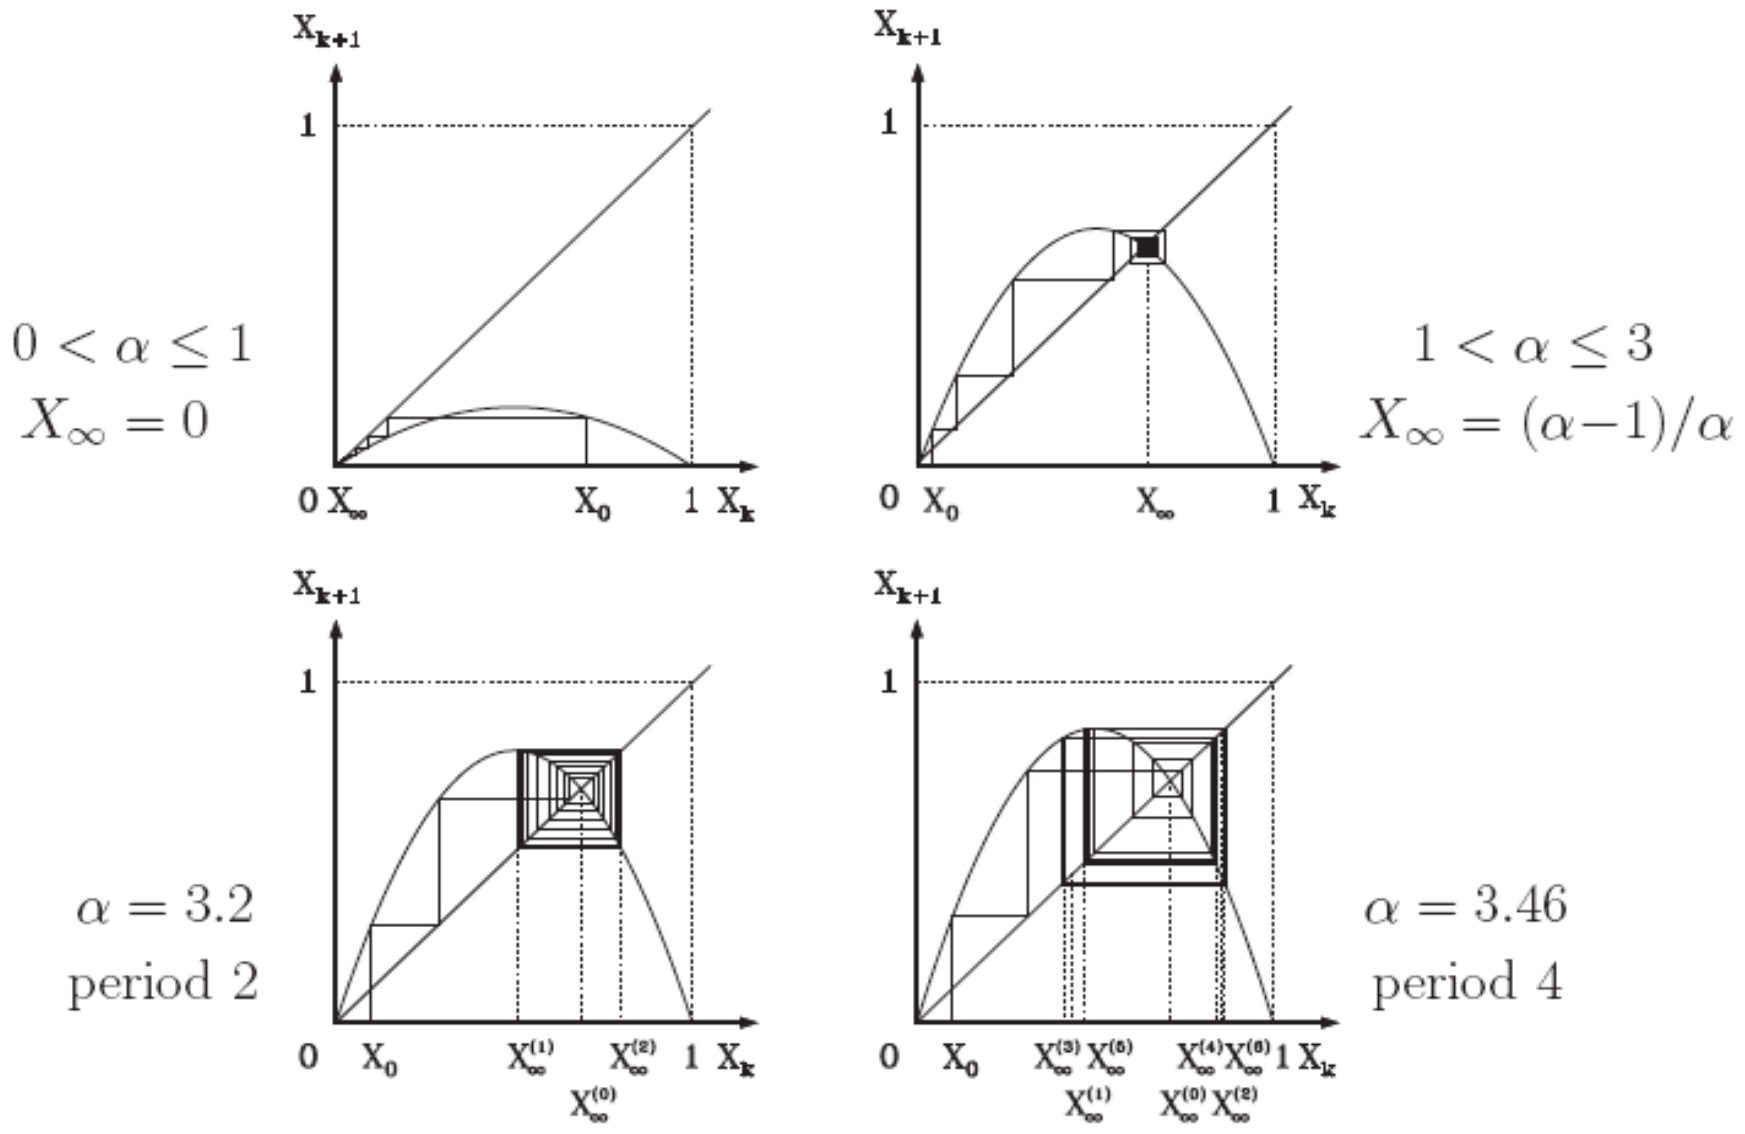
\includegraphics[width=0.7\textwidth]{Pictures/chaos_theory_intuition.png}
\end{figure}

\begin{figure}[H]
    \centering
    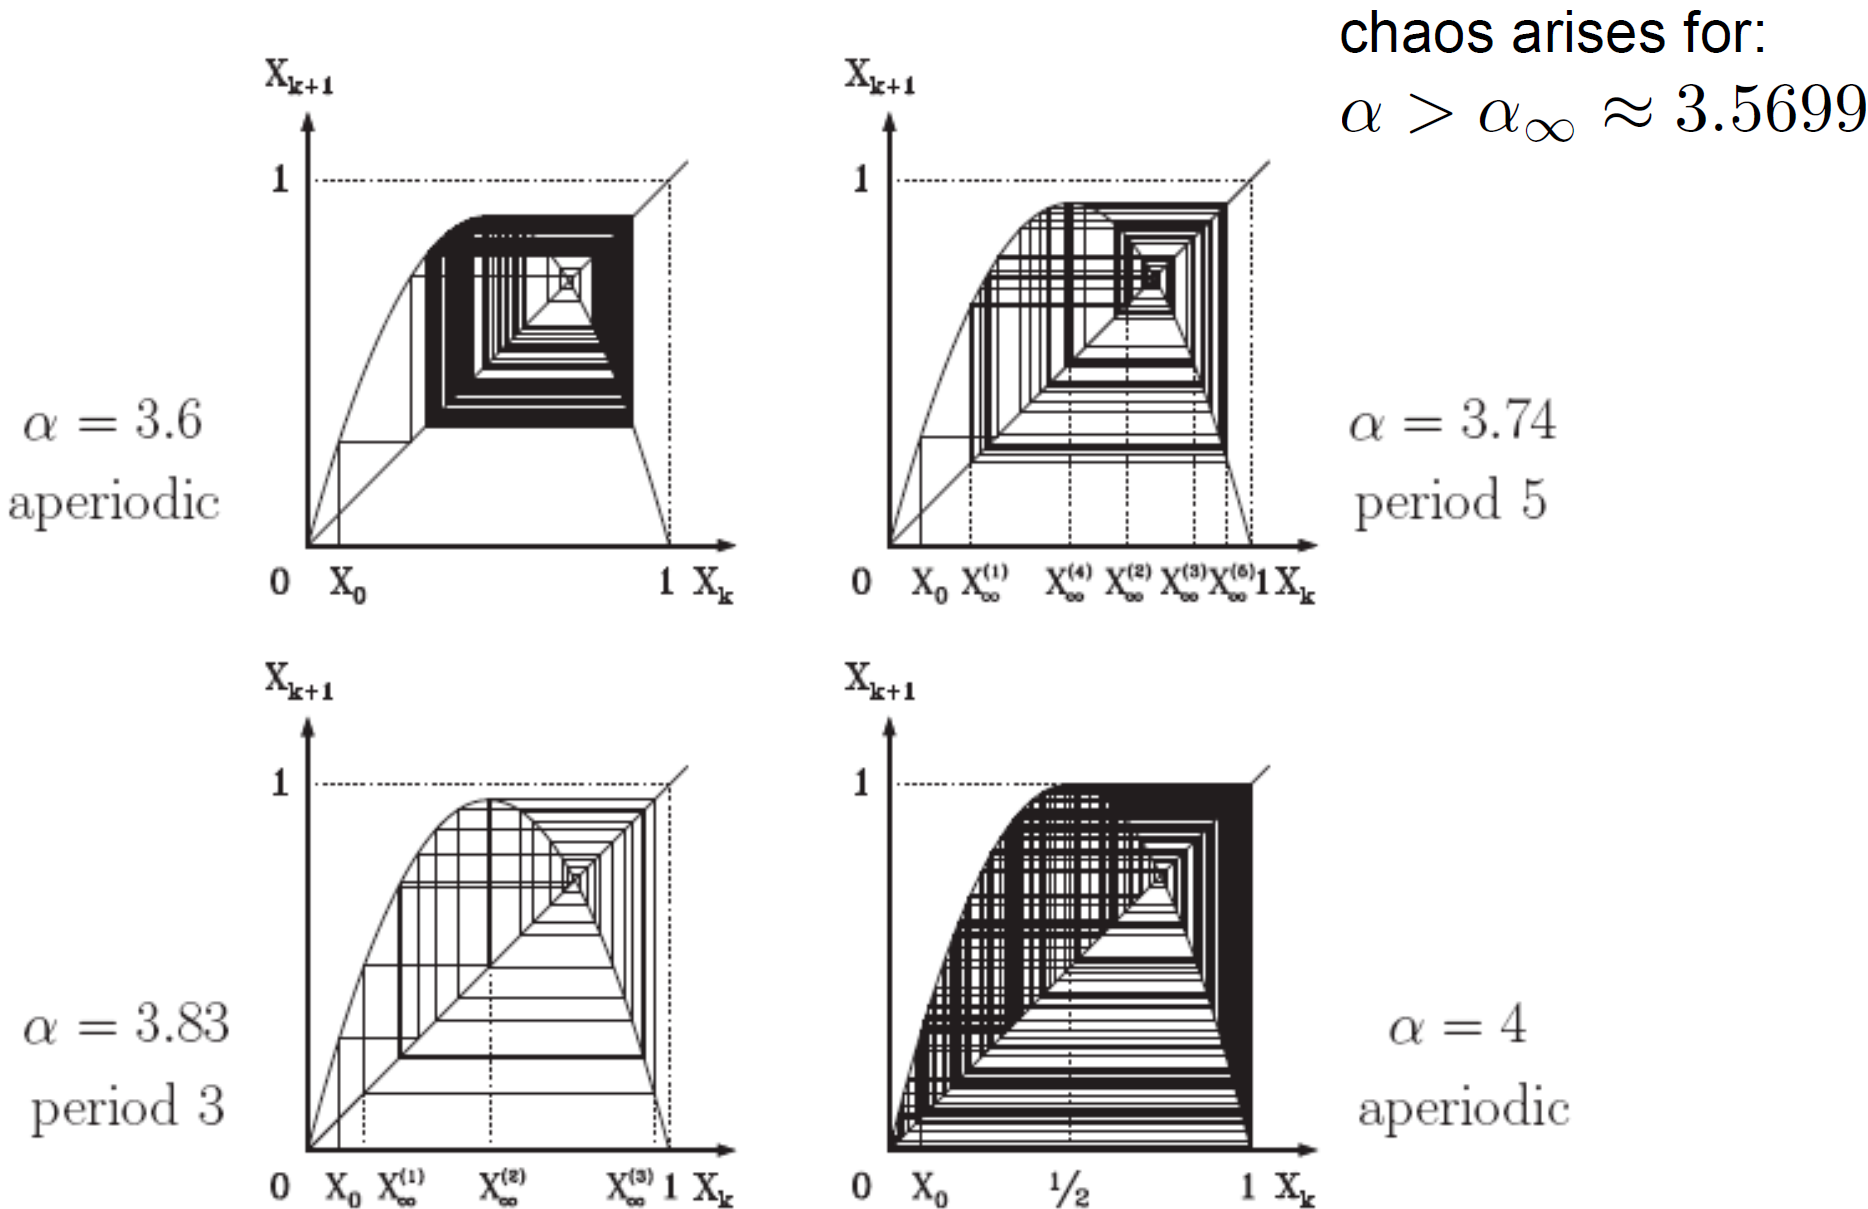
\includegraphics[width=0.7\textwidth]{Pictures/chaos_theory_intuition_2.png}
\end{figure}

\pagebreak

\paragraph{Bifurcation diagram}

\begin{figure}[H]
    \centering
    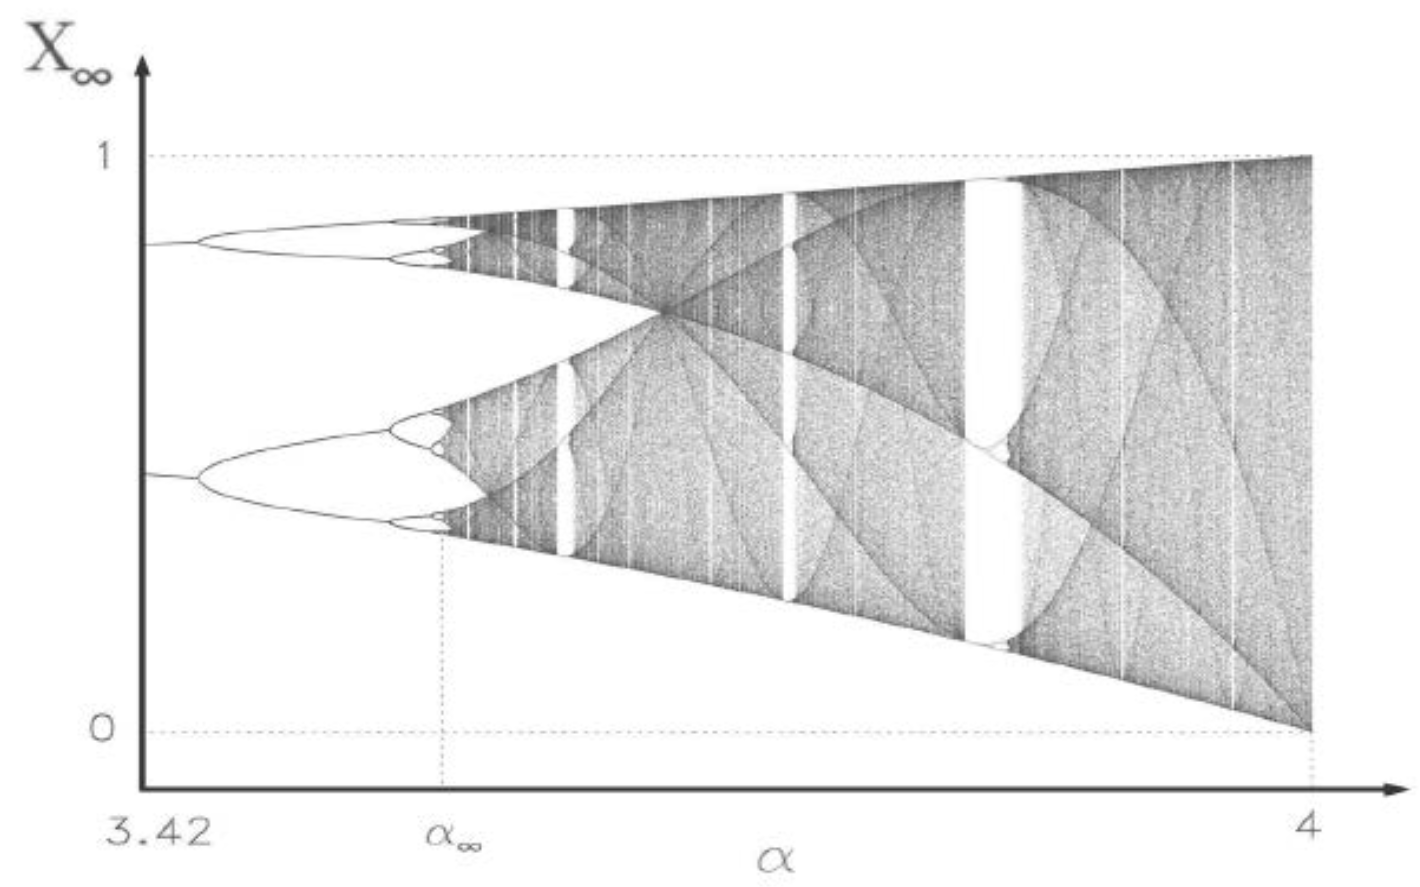
\includegraphics[width=0.7\textwidth]{Pictures/logistic_map_bifurcation_diagram.png}
    \caption{Bifurcation diagram}
\end{figure}

After $\alpha_\infty$, dusty "strange attractors" are common expansion of periodic
buds gives small copies of tree!


\subsubsection{Number Theory: roots of randomness}

It can be shown that the logistic map is equivalent to the tent map
\begin{align*}
    y(n+1) = 2y(n) \ \mod{1}
\end{align*}
with $x_n = \sin^2(2 \pi y_n)$ and $\alpha = 4$.
This explains the origin of the chaotic behaviour as fundamentally
embedded the mathematical properties of the digits of irrational numbers,
which are of measure $1$ among real numbers.

\subsubsection{Chaos}

\paragraph{Definition}
Chaos is not random, but due to a deterministic map $x: A \rightarrow B$
satisfying the following properties:
\begin{enumerate}
    \item $x$ is low dimensional
        \begin{itemize}
            \item $x$ is only dependent on a "small" number of variables,
                for instance: $x(n+1) = f(x(n),x(n-1),x(n-2))$. Nevertheless,
                the outcome is very complex!
        \end{itemize}
    \item $x$ is deterministic
        \begin{itemize}
            \item This means, that the next value can always be predicted exactly.
        \end{itemize}
    \item $x$ is sensitive to initial values
        \begin{itemize}
            \item Slight changes in the initial value can dramatically change
                the output.
        \end{itemize}
    \item trajectories of $x$ are reinjected
        \begin{itemize}
            \item Although slight differences in initial values $x1$ and $x2$
                lead to trajectories which can be arbitrarily far apart from
                each other, there will be a point at which these two trajectories
                are again arbitrarily close to each other.
        \end{itemize}
\end{enumerate}

\pagebreak

\subsection{The diffusion of innovation}

Focus questions: How does a new technology spread? How are new products
adopted by people in society?

\paragraph{Categories of adoption}

There are five different categories:

\begin{figure}[h]
    \centering
    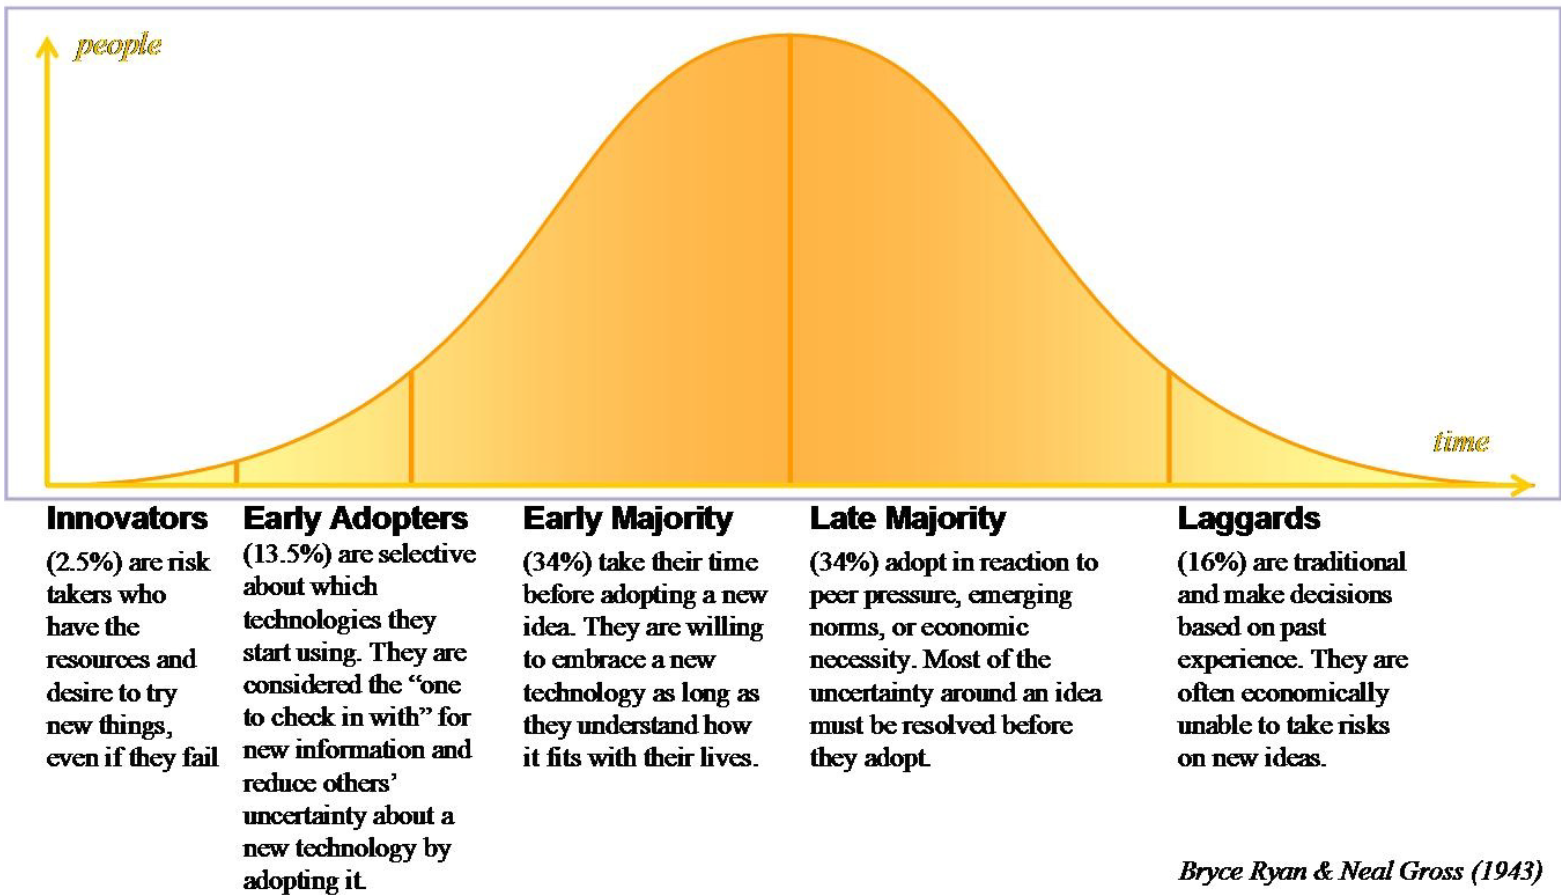
\includegraphics[width=0.7\textwidth]{Pictures/Categories_of_adoption.png}
\end{figure}

\paragraph{Terminology}

\begin{enumerate}[]
    \item \underline{Penetration rate}: The penetration rate is like the
        population size in Part \uproman{1}, it follows an S-shaped curve
        and saturates at 100\% when the full population has adopted the new
        technology.
    \item \underline{Penetration speed}: The penetration speed is comparable
        to the production rate, it follows a Gaussian shaped curve.
\end{enumerate}

\subsubsection{The Agent Based Model (ABM) of Namatame}

\paragraph{Definitions}

\begin{itemize}
    \item $F(t)$ is the \underline{penetration rate}, it is the fraction
        of the population that has adopted the new technology, this will
        follow an S-shaped curve, it is cumulative.
    \item $F(t+1) - F(t)$ is the penetration speed, it is the fraction
        of the population that adopts the new technology in the following
        time-step, this will follow a Gaussian-shaped curve.
    \item $p(t+1)$ gives the probability that an agent will adopt the new
        technology in the next time-step.
\end{itemize}

\begin{figure}[h]
    \centering
    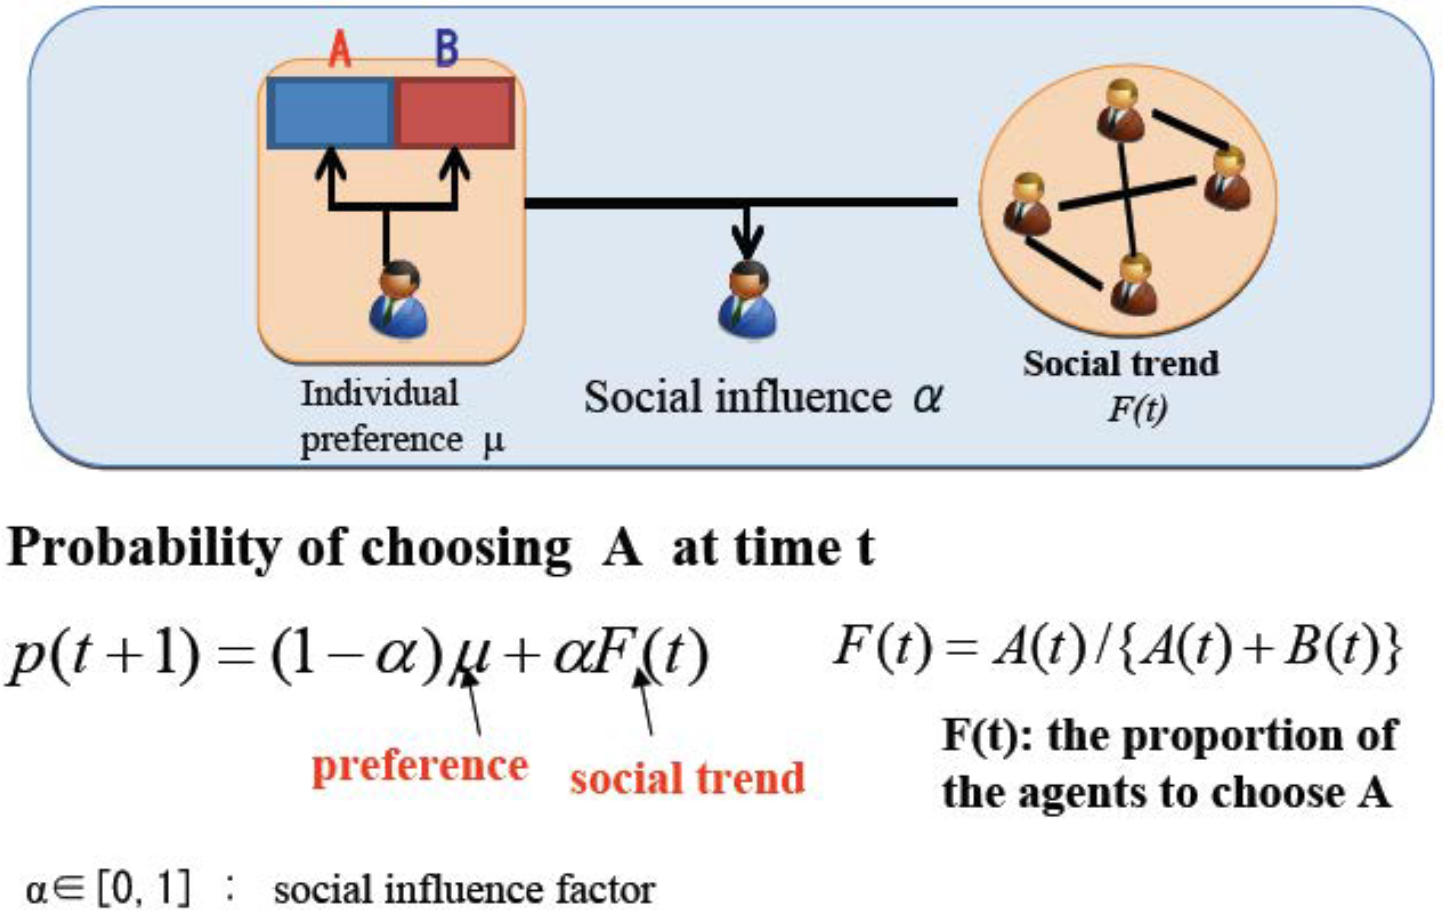
\includegraphics[width=0.55\textwidth]{Pictures/ABM_1.png}
\end{figure}

\paragraph{The Model}

\begin{itemize}
    \item $p(t+1) = (1 - \alpha) \mu + \alpha F(t)$. The first term corresponds
        to personal preferences (is a constant) and the second term corresponds
        to the social trend (A fraction of the penetration rate, the social
        trend increases as more people adapt).
    \item $p(t+1)$ only applies to agents that have not yet adopted, this
        concerns the fraction $(1-F(t))$ of the agents.
    \item As a consequence: $F(t+1) - F(t) = p(t+1) \cdot (1-F(t))$.
        The penetration rate is the probability that an agent adapts times
        the number of non-adapted agents.
    \item $F(t+1) = F(t) + p(t+1) \cdot (1-F(t)) = F(t) +
        \klammer{(1-\alpha) \cdot \mu + \alpha \cdot F(t)} \cdot (1-F(t))$
    \item In case there is no personal preference and only social interaction:
        \begin{itemize}
            \item $\mu = 0$
            \item $F(t+1) = F(t) + \alpha \cdot F(t) \cdot (1 - F(t))$
            \item In continuous form:
            \begin{itemize}
                \item $\frac{dF(t)}{dt} = \alpha \cdot F(t) \cdot (1 - F(t))$
                \item This is the logistic differential equation with $K=1$
                \item 100\% penetration rate agrees with a carrying capacity of 1
                \item $r = \alpha$
            \end{itemize}
        \end{itemize}
    \item In the case there is only personal preference, and no social
        interaction or context:
        \begin{itemize}
            \item $\alpha = 0$
            \item $F(t+1) = F(t) + \mu \cdot (1 - F(t))$
            \item continuous form:
            \begin{itemize}
                \item $\frac{dF(t)}{dt} = \mu \cdot (1 - F(t))$
                \item $F(t) = 1 - \exp(-\mu \cdot t)$
            \end{itemize}
            \item This is like radioactive decay, the concentration of
                the parent nuclei drops exponentially and the concentration
                of the doughter nuclei increases with $1 - \exp$. Indeed
                there is no interaction between the nuclei in radioactive
                decay.
        \end{itemize}
    \item The penetration rate differs for different levels of social
        interaction and varies between a process without any social
        interaction, like nuclear decay, and a process with a very strong
        social interaction, like the growth of rabbits.
\end{itemize}

\paragraph{Example: Diffusion of innovation}

Penetration rate as a function of time, more like a step function means more
social interaction, or more trendy products. If the diffusion speed is
parabolic, there is social interaction and if it is linear, there is no
social interaction.

\subsection{Case Study - the valuation of the company Facebook before the IPO}

Analysis: see Lecture slides of Lecture 6 on 14/04/2021.
\footnote{\url{https://xyotta.com/cfiles/1186}}

\paragraph{Greenshoe option}
\begin{itemize}
    \item A greenshoe option is also called an over-allotment option:
    \item At the IPO, the underwriters sold 15\% more shares then what was
        initially targeted, creating a big short position (2.4 billion USD)
    \item If the price goes up, covering this short would be extremely expensive
    \item When the underwriters execute the greenshoe option, Facebook must
        emit 15\% more shares at the IPO price. This allows them to cover their
        position without any loss.
    \item If the price goes below the IPO price, they can close the short
        position, buy back the shares at the IPO price and as such support
        the price at the IPO level.
\end{itemize}

Putting aside the fact that Facebook was hugely overvalued (and was for
a long time), reports about reduction of revenues estimates were withheld
before the IPO from retail investors. Instead of decreasing the price of
the IPO in view of the worse financials, the price was increased from
28\$-35\$ to 34\$-38\$. The IPO was at 38\$. Instead of decreasing the
volume of the IPO, it was increased from 337 million shares to 421 million
(+25\%). It was hoped that the deal could be shoved down the throught of
retail investors who would buy it because of the brand name. It didn't work,
they went a bridge too far.

\subsubsection{Ex-ante prediction}

\begin{itemize}
    \item On the long term, the market price should converge to the
        fundamental one.
    \item This is not necessarily true on the short term: the market can
        stay crazy longer than you can stay solvent\dots
    \item Predictions made were correct due to two main events:
        \begin{enumerate}
            \item A quarterly financial report was coming out on April 26th.
                From our fundamental analysis, we knew that the revenues were
                saturating. We therefore expected a downward move in price
                following the results.
            \item On April 30th, the lock-up period expired, adding 115 million
                shares to the 150 million shares already on the market. We
                expected the overvaluation of Zynga to be reflected in its
                market price as soon as insiders, better informed about the
                fundamental of their company, would begin to trade.
        \end{enumerate}
    \item This gave rise to a trading strategy based on 3 legs:
        \begin{enumerate}
            \item From the time of writing (April 16, 2012) the announcement
                of the financial results (around April 26, 2012): stay out
                of Zynga or hedge if invested.
            \item From the day after the earnings announcement (around April 27,
                2012) to the end of the first lock-up period (around April 30, 2012):
                if the financial results are significantly above those of the previous
                quarter, buy Zynga for a short-term holding period; otherwise short it.
            \item From the end of the first lock-up period (after 30 April, 2012):
                close all open long positions and short. Monitor the subsequent quarterly
                releases and the successive ends of future lock-up periods to position
                a strategy in the same spirit as above.
        \end{enumerate}
\end{itemize}

\subsubsection{Conclusion}

\begin{itemize}
    \item We have developed a new methodology to compute the fundamental
        value of social networking companies based on the dynamics of their
        users' and revenues per user. Based on that, we can compute the
        intrinsic value of social networking companies.
    \item The intrinsic value is not only useful to make long term predictions.
        When coupled with the right information (financial report, lock-up
        expiration) it might enable us to make shorter term predictions. We
        need to test this hypothesis on a statistical basis.
    \item Bubbles are great for innovation and crossing capital and risk
        hurdles. But they are bad for capital allocation.
\end{itemize}

There are three important laws of valuation and investment:
\begin{enumerate}
    \item Prediction is not extrapolation, understanding the underlying
        process. Example: the logistic function is exponential in the
        beginning but plateaus after the inflection point.
    \item Unterstand the technicalities of the market and of investment
        banking. Example 1: the flat price 38 was a clear signal that the
        price was srtificially supported by the testosterone of the
        greenshoe. Example 2: who are the buyers/sellers? The retail IPO
        was an attempt to sell the brand and shovel the deal down the
        throat of the users.
    \item Always RTFM - Read the fucking Manual! Example: When does the
        lock-up period end? The moment when the insiders can start selling?
\end{enumerate}

